% !TeX program = pdflatex
\documentclass[a4paper,11pt]{article}
\usepackage[T1]{fontenc}
\usepackage[utf8]{inputenc}
\usepackage{lmodern}
\usepackage[margin=25mm]{geometry}
\usepackage{amsmath,amssymb,bm}
\usepackage{graphicx,booktabs,tabularx,array}
\usepackage[numbers,sort&compress]{natbib}
\usepackage{microtype}
\usepackage{placeins}
\usepackage[colorlinks=true,linkcolor=blue,citecolor=blue,urlcolor=blue]{hyperref}
\usepackage{url}
\urlstyle{tt}
\setlength{\emergencystretch}{4em}
\setlength{\parskip}{0.25em}
\setlength{\parindent}{1em}
\renewcommand{\arraystretch}{1.18}
\newcolumntype{Y}{>{\raggedright\arraybackslash}X}
\graphicspath{{figures/}}
\hypersetup{pdfauthor={Chengheng}}

\title{Conditional Robustness of Binary-Black-Hole Population Inference\\[0.4em]\large Reproducible diagnostics of prior support, injection provenance, and shared-sample Monte Carlo uncertainty}
\author{Chengheng\\\small Blackhole Research Workbench}
\date{24 October 2026\\\small v0.2 --- Not peer reviewed}
\begin{document}
\maketitle
{\small Manuscript status: public technical research draft, not peer reviewed. Chengheng is the pen name used by the collaborating AI assistant (ChatGPT, OpenAI) in this project. No human accountable author has been designated. This attribution does not imply institutional endorsement by OpenAI. Code and calculated results: \href{https://github.com/wkryyds4-netizen/blackhole-research-workbench}{project repository}.\par}
\begin{abstract}
The population distribution of binary-black-hole spin tilts can constrain formation scenarios, but interpreting a finite gravitational-wave sample in terms of formation-channel fractions depends on population models, observational selection, and numerical integration. Using a conditional 69-event baseline from the public GWPopulation tutorial, we separately examine the distinction between a mixture parameter and a common physical functional, the provenance and measure consistency of injection data, and correlated Monte Carlo errors induced by reusing samples across models. We compute the intrinsic fraction of primary black holes with negative spin-tilt cosine across 81 fixed hyperparameter settings and match its prior support within 27 triplets of tilt-width models. Only nine triplets show substantially reduced median dispersion, and all nine coincide with failures of the adopted pointwise numerical screen. We recover exact row-level correspondence for all 41,972 retained injections to an official source HDF, including run labels, a reproducing selection mask, and the sampling-density transformation. Across six representative settings, restoring near-unity run-mixture weights produces a maximum computed common-prior median shift of approximately 6.65\(\times\)10\textsuperscript{-9}. In 2,048 empirical resamples with shared counts, the baseline spin-amplitude model retains a 6.734 percentage-point difference between \(\sigma\)=0.3 and 1.2, with a 5th–95th percentile resampling range of 5.557–7.600 points. The corresponding low-spin stress case has a difference of 1.115 points and a range of \(-\)0.293–3.601 points. These ranges quantify empirical numerical sensitivity, not astrophysical credible intervals. A common prior does not automatically remove model dependence, and pointwise likelihood variance cannot replace posterior-shape diagnostics. We provide reproducible conditional robustness experiments and a provenance audit, without claiming a model-independent tilt measurement or formation-channel fractions.
\end{abstract}
\noindent \textbf{Keywords:} gravitational waves; binary black holes; population inference; selection effects; spin tilts; importance sampling; reproducible research\par
\FloatBarrier
\section{Introduction}\label{sec:1}
Binary black holes can form through stellar binary evolution, dynamical interactions in dense stellar clusters, and evolution and mergers in other environments. These scenarios may predict different masses, spin magnitudes, spin directions, redshift evolution, and eccentricities. Detectors do not directly provide formation labels. Observations first yield source-parameter posteriors with substantial uncertainty, and population models are then used to interpret the event ensemble. A single phenomenological component generally does not correspond one-to-one to a single astrophysical channel \cite{ref1}.

Spin tilts provide a useful test of this problem. A component concentrated near alignment with the orbital angular momentum often represents an alignment-favoring population, while an isotropic component represents dispersed directions. These descriptions do not uniquely identify an astrophysical origin. The location, shape, and evidence for a tilt peak depend on the model and prior, as previous studies have explicitly discussed \cite{ref2}. More recent work examines integrals over angular intervals and degeneracies between effective-spin constraints and component-spin models \cite{ref5,ref6}.

Event integrals and search-sensitivity integrals in a hierarchical likelihood are usually evaluated by importance reweighting finite samples. Numerical errors depend on effective sample size and are correlated between hyperparameter points that reuse the same samples \cite{ref3,ref4}. Treating these errors as independent can misrepresent differences between models. Conversely, inspecting only pointwise log-likelihood variance can mistake a common shift, which posterior normalization removes, for a change in posterior shape.

We do not present the existence of model dependence, the interpretability of integrated functionals, or the importance of selection effects as new theoretical discoveries. Our aim is to implement these known issues in a concrete, publicly reproducible analysis and answer three limited questions. Do differences between fixed models remain when the target quantity and its prior support are matched? How far can the provenance and selection rules of tutorial preprocessing be recovered? Which model differences persist under shared-sample empirical perturbations, and which readily change ordering?

The contributions are an experiment distinguishing parameter transformations from prior controls, row-level provenance recovery for 41,972 public injections, and paired empirical resampling of six settings with independent mathematical checks. Because the complete event parameter-estimation provenance and the actual injection-generation design have not been recovered, we restrict our conclusions to conditional diagnostics and do not infer physical formation-channel fractions.

\FloatBarrier
\section{Data, versions, and scope}\label{sec:2}
\subsection{Tutorial event baseline}\label{sec:2.1}
The preprocessed posterior and injection data come from the public GWTC-3 tutorial of GWPopulation \cite{ref7}. The tutorial supplies 73 event arrays. Our project retains 69 groups using a secondary-mass posterior median greater than 3 solar masses and catalog FAR below 1 per year. The earlier code temporarily retained ten entries with missing FAR; subsequently recovered search records confirm that all ten satisfy the threshold. The retained groups contain 476,997 posterior samples. The arrays contain source-frame primary mass, mass ratio, redshift, two spin magnitudes, two tilt cosines, and numerical prior densities. Importance reweighting uses the full-dimensional samples, without replacing event posteriors by catalog medians.

The preprocessed arrays do not retain original event names. Current labels were reconstructed by one-to-one matching of catalog mass, effective-spin, and redshift summaries, with an additional check on time ordering. Event names in this paper are therefore reconstructed metadata. This procedure does not establish the identities, waveform models, priors, or versions of the original parameter-estimation (PE) files.

A historical audit of the tutorial code shows successive removal of indices 15 and 38. The second index is measured after the first removal, so the original indices are 15 and 39, leaving 71 entries. Our project additionally excludes two entries with FARs of 3.3 and 4.8 per year, leaving 69. Agreement in sample size with another 69-event study does not establish identical membership or waveform settings. This is not a complete reproduction of an official LVK population result.

\subsection{Separating search significance from PE records}\label{sec:2.2}
The initial audit found empty FAR fields for ten GWTC-1 binary black holes. The cause was catalog merging: newer GWTC-2.1 records, keyed by event name, overwrote nonempty older search values with empty FAR fields. Restoring the GWTC-1 source shows that all ten meet the current FAR<1 per year condition; event membership is unchanged.

This repair demonstrates why PE updates and search-significance information require separate provenance fields. A newer record cannot automatically be assumed to be more complete in every field. Missing FAR must not automatically be interpreted as either passing or failing a threshold. We preserve the earlier inference and record the repair as a separate audit product.

\subsection{Injection file and frozen input}\label{sec:2.3}
The local injection array contains 41,972 retained samples, with a total normalization of 73,280,198 and an analysis duration of 2.000455579638502 years. Stage two establishes an exact correspondence to the BBH file in the official O1+O2+O3 search-sensitivity release \cite{ref8}. The original HDF is 63,149,928 bytes and has the official MD5 c21337a25b7318fdfd471cce549a547e. The 2021 and 2023 release records list the same checksum for this file.

The main statistical experiment freezes \path{results/model.json}, whose SHA-256 is given in Appendix A. This file stores event and injection weight moments for 81 settings. Before resampling, we recompute the raw weights for six settings from local safe NPZ arrays and confirm exact agreement with the frozen moments. The earlier event list, inference, and raw arrays are preserved.

\subsection{Meaning of the target quantities}\label{sec:2.4}
The primary quantity is the intrinsic population fraction of primary black holes r=P(cos \(\theta_{1}\)<0), corresponding to a spin–orbital-angular-momentum angle greater than 90\({}^\circ\). It is not a direct frequency in the detected sample, the fraction of binaries with at least one such component, or the branching fraction of a formation channel. The secondary functional \(F_{10}\)=P(\(\theta_{1}\)<10\({}^\circ\)) is used to examine the information properties of coordinate transformations.

\FloatBarrier
\section{Conditional population model and likelihood}\label{sec:3}
\subsection{Population distribution}\label{sec:3.1}
Let \(c_{i}\)=cos \(\theta_{i}\). The joint tilt model mixes an alignment-favoring truncated Gaussian with an isotropic component:

\begin{equation}\label{eq:1}
p(c_1,c_2|f,\sigma)=f A_\sigma(c_1)A_\sigma(c_2)+(1-f)/4.
\end{equation}
\begin{equation}\label{eq:2}
A_\sigma(c)=\frac{\exp[-(c-1)^2/(2\sigma^2)]}{\sigma\sqrt{2\pi}\,[\Phi(0)-\Phi(-2/\sigma)]},\quad -1\leq c\leq1.
\end{equation}
Both black holes share one mixture-component label; they do not independently select a component with probability f. Tilts are conditionally independent within a component, but the mixture is generally not independent. The mass, spin-amplitude, and redshift factors are the same in both tilt components and factorize from the tilts.

The source-frame primary-mass model mixes a power law p(\(m_{1}\)) proportional to \(m_{1}\) raised to \(-\)\(\alpha\) over 3–100 solar masses with a truncated Gaussian peak. The peak has mean 35 solar masses and standard deviation 5 solar masses. For mass ratio q between 3/\(m_{1}\) and 1, p(q|\(m_{1}\)) is proportional to q. Both spin magnitudes follow the same Beta distribution. The redshift distribution over 0–2.3 is proportional to the Planck15 comoving-volume element multiplied by (1+z) raised to \(\lambda\)\(-\)1.

Table~\ref{tab:1} lists the fixed settings. They define 81 conditional analyses, not joint sampling of these hyperparameters. No model-probability weights are assigned to the 81 settings.

\begin{table}[tbp]
\centering\small
\caption{Fixed settings defining the 81 conditional analyses.}\label{tab:1}
\begin{tabularx}{\linewidth}{Y Y c}
\toprule
Variation axis & Fixed candidate values & Count \\
\midrule
Tilt width \(\sigma\) & 0.3; 0.6; 1.2 & 3 \\
Spin-amplitude Beta shape parameters & (1.5,8.5); (2,5); (1,1) & 3 \\
Primary-mass power-law index and peak weight & (2,0.1); (3,0.1); (2,0) & 3 \\
Redshift evolution \(\lambda\) & 0; 2; 4 & 3 \\
\bottomrule
\end{tabularx}
\end{table}
\subsection{Selection correction conditional on the event count}\label{sec:3.2}
For event i, the stored posterior samples \(\theta_{ij}\) come from PE under reference prior \(\pi_{i}\). Omitting the event evidence, which is independent of population parameters, the event integral is estimated as

\begin{equation}\label{eq:3}
\widehat{\mu}_i(\Lambda)=\frac{1}{n_i}\sum_{j=1}^{n_i}\frac{p(\theta_{ij}|\Lambda)}{\pi_i(\theta_{ij})}.
\end{equation}
For retained injections \(\theta_{k}\) with sampling density \(q_{k}\), the original baseline estimates the search efficiency and conditional log likelihood as

\begin{equation}\label{eq:4}
\begin{aligned}\widehat{\xi}(\Lambda)&=\frac{1}{N_{\rm gen}}\sum_{k\in{\rm found}}\frac{p(\theta_k|\Lambda)}{q_k},\\\log\widehat{\mathcal L}&=\sum_{i=1}^{N}\log\widehat{\mu}_i-N\log\widehat{\xi}.\end{aligned}
\end{equation}
We fix N=69 and do not infer an absolute merger rate. The numerical prior columns are those supplied by the preprocessing. The injection-side measure is recovered in Section~\ref{sec:5}; the complete original event-side prior configuration remains unverified. The original baseline omits the subsequently recovered run-mixture weights. Section~\ref{sec:5.3} evaluates that correction separately.

Because f mixes two components linearly, each event mean and the selection efficiency are linear combinations of two fixed component values. Stored first and second moments therefore allow exact reconstruction of this model's one-dimensional conditional likelihood and facilitate comparisons using the same samples.

\FloatBarrier
\section{Functionals, prior support, and information invariance}\label{sec:4}
\subsection{From a mixture parameter to a common physical quantity}\label{sec:4.1}
Writing \(B_\sigma\) for the CDF of \(A_\sigma\), the primary-black-hole marginal gives

\begin{equation}\label{eq:5}
r(f,\sigma)=\frac{1}{2}+f\,[B_\sigma(0)-\frac{1}{2}].
\end{equation}
\begin{equation}\label{eq:6}
F_{10}(f,\sigma)=u+f(v_\sigma-u),\quad u=\frac{1-\cos10^\circ}{2},\quad v_\sigma=1-B_\sigma(\cos10^\circ).
\end{equation}
We first evaluate r or \(F_{10}\) at each population-parameter point and then calculate its posterior quantiles. Integrating the posterior-averaged population predictive distribution gives only the posterior mean of a functional, not its full uncertainty.

For fixed finite \(\sigma\), Equations~\eqref{eq:5} and~\eqref{eq:6} are one-to-one affine transformations of f. Transforming both posterior and prior densities correctly leaves their KL divergence unchanged:

\begin{equation}\label{eq:7}
D_{\rm KL}(p_r\Vert\pi_r)=D_{\rm KL}(p_f\Vert\pi_f).
\end{equation}
The absolute mean shift normalized by the prior standard deviation and the ratio of posterior to prior standard deviation are also unchanged. Thus, a numerically narrower r interval at the same fixed \(\sigma\) does not establish additional information. If \(\sigma\) is free, the mapping is generally no longer one-to-one and this invariance argument cannot be applied directly. Our fixed-model diagnostic does not negate the interpretive value of functionals in studies with multiple model families and free hyperparameters \cite{ref5}.

\subsection{Shared-support control}\label{sec:4.2}
The original prior is uniform in f on \([0,1]\). The three widths induce r supports of [0.000858,0.5], [0.094804,0.5], and [0.341740,0.5]. To control this difference, we define a separate common interval:

\begin{equation}\label{eq:8}
R=[\max_\sigma B_\sigma(0),\,1/2]=[0.341739786994,\,0.5],\quad \pi_R(r)={\rm Uniform}(R).
\end{equation}
We compare the three \(\sigma\) values at fixed spin-amplitude, mass, and redshift settings, giving 27 triplets. This is a prior-changing control that deliberately removes part of the previously allowed r domain, not an unconditional improvement to the prior. We record the original prior and posterior mass retained in R. Only the marginal prior on r is matched; neither the \(F_{10}\) prior nor the full tilt distribution is claimed to be matched.

The model itself excludes r>0.5. Under a continuous prior, f=0 is the isotropic boundary point and has zero prior probability mass. An equal-tailed interval excluding r=0.5 does not automatically provide evidence against isotropy. We do not perform model comparison for that discrete hypothesis.

\subsection{Pointwise numerical screen}\label{sec:4.3}
The inherited exploratory thresholds require a minimum effective sample size of 50 for every event, an injection effective sample size of at least 4N, and a delta-method log-likelihood standard deviation no greater than 1. We record the prior and posterior mass passing these thresholds and the common passing domain of each model triplet.

\begin{equation}\label{eq:9}
n_{\rm eff}=n\frac{\overline{w}^{\,2}}{\overline{w^2}}.
\end{equation}
For injection ESS, n in Equation~\eqref{eq:9} is the local Ngen, not the detected count M. The averages include the collapsed zero-weight entries. The expression is equivalent to the squared sum of detected weights divided by their sum of squares. Here Ngen serves only as the effective denominator of the original estimator.

These thresholds locate numerical risks; they are not used to remove parameter points and renormalize the posterior. Failing a threshold does not exclude a physical model, and passing does not establish control of bias. Correlated errors, missed tails, and the actual sampling mechanism require further examination \cite{ref3,ref4}.

\FloatBarrier
\section{Injection provenance and deterministic weight controls}\label{sec:5}
\subsection{Row identities and selection mask}\label{sec:5.1}
The official source file contains 289,620 retained injections. Primary masses alone are not unique, so we match using exact pairs of primary mass and redshift. After confirming uniqueness of all source-file keys, we compare the remaining coordinates element by element. All 41,972 local samples match uniquely in the same order; all seven physical-coordinate columns satisfy strict equality.

On this HDF, the following rule exactly reproduces the local retained set: IFAR>1 year in any of five search pipelines, or membership in O1/O2 with optimal network SNR>10. The searches are cWB, GstLAL, MBTA, PyCBC BBH, and PyCBC hyperbank. The symmetric difference between this mask and the local set is zero. Table~\ref{tab:2} gives the run counts.

\begin{table}[tbp]
\centering\small
\caption{Run membership and recovered injection mixture weights.}\label{tab:2}
\begin{tabularx}{\linewidth}{l r r Y}
\toprule
Run & Retained rows in source HDF & Local detected rows & Per-row run-mixture weight \\
\midrule
O1 & 51194 & 1623 & 1.0000057241333624 \\
O2 & 109972 & 3881 & 0.9999982192691211 \\
O3 & 128454 & 36468 & 0.9999992049793384 \\
\bottomrule
\end{tabularx}
\end{table}
Retained HDF rows are not the total number of simulated draws for a run. Recovering the exact selected set in a finite file does not uniquely recover the historical thresholds, preprocessing command, or software version: multiple thresholds within gaps of the statistic can select the same rows.

\subsection{Density transformation and effective normalization}\label{sec:5.2}
After changing from two source-frame masses to primary mass and mass ratio, transforming Cartesian spins to amplitudes and tilt cosines, and integrating out azimuths, the local prior equals the following expression element by element:

\begin{equation}\label{eq:10}
q_{\rm local}=q_{\rm Cartesian}\,m_1(2\pi a_1^2)(2\pi a_2^2).
\end{equation}
This establishes the injection-side coordinate-measure conversion. The original HDF reports total\_generated=73280198.73534885; the local value is its integer truncation. The original analysis duration of 63,129,577 seconds exactly matches the local duration when converted using 365.25 days per year. The noninteger total is official effective-normalization metadata; it cannot be interpreted directly as an established integer count of IID trials.

\subsection{Effect of the omitted mixture weights}\label{sec:5.3}
The official documentation treats sampling\_pdf and mixture\_weight as separate fields, with the latter included in the Monte Carlo sum \cite{ref8,ref9}. The local prior does not absorb this weight. We therefore multiply the recovered weights into the injection importance-sampling terms while leaving event integrals unchanged.

For nonnegative population weights, the efficiency ratio after and before this correction lies between the minimum and maximum mixture weights. Consequently, for the conditional 69-event likelihood, the following bound on the range of the log-likelihood correction holds for any such population weights:

\begin{equation}\label{eq:11}
\operatorname{range}(\Delta\log\mathcal L)\leq N\log(w_{\max}/w_{\min})=5.18\times10^{-4}.
\end{equation}
Across the six representative settings, the largest computed median shift is 6.65\(\times\)10\textsuperscript{-9} under the common r prior and 3.65\(\times\)10\textsuperscript{-8} under the original induced priors. The correction differs by less than 1.88\(\times\)10\textsuperscript{-11} between 4001-point and 8001-point quadrature. Restoring the noninteger total changes only a parameter-independent selection-normalization constant. The conditional posterior is unchanged to floating-point precision, with numerical total variation 1.52\(\times\)10\textsuperscript{-14}.

The recovered near-unity run-weight omission and total truncation therefore cannot explain the percentage-point-scale model differences. This excludes two specific explanations only. Incorrect event priors, inconsistent selection policies, and actual injection sampling errors are not bounded by Equation~\eqref{eq:11}.

\FloatBarrier
\section{Paired empirical resampling with shared samples}\label{sec:6}
\subsection{Representative settings and stochastic mechanism}\label{sec:6.1}
Stage two fixes six settings: each of the three \(\sigma\) values with either low spin amplitudes Beta(1.5,8.5) or baseline amplitudes Beta(2,5), holding the mass setting at (2,0.1) and \(\lambda\)=2. The low-spin group was selected from stage-one low-ESS cases, and the other group is the original baseline. This selection is documented. All settings use the common prior in Equation~\eqref{eq:8}.

For each event, we draw multinomial counts for \(n_{i}\) draws among its original \(n_{i}\) samples. For injections, we construct an empirical vector of M=41972 stored weights and Ngen\(-\)M zero weights, collapsing all zero entries into a single category:

\begin{equation}\label{eq:12}
\boldsymbol{C}\sim{\rm Multinomial}\left(N_{\rm gen};\frac{1}{N_{\rm gen}},\ldots,\frac{1}{N_{\rm gen}},1-\frac{M}{N_{\rm gen}}\right).
\end{equation}
The counts for a given event or injection are shared across all six models and all r points. Different events, and the event and injection draws, are independent. Catalog membership remains fixed; we do not resample the event list. We run three modes: perturbing event integrals only, injection integrals only, or both. Seeds 20261024 and 20261025 each provide 1024 repetitions, for 2048 in total. Each repetition renormalizes the conditional posterior and extracts its quantiles.

Equation~\eqref{eq:12} explicitly uses the local integer Ngen=73280198. The original noninteger normalization is used only in the deterministic control of Section~\ref{sec:5.3}. Equation~\eqref{eq:12} defines a specific empirical perturbation mechanism, not the actual repeated-sampling mechanism of the original campaigns: the original effective total is noninteger, the run-mixture design is incompletely recovered, and chain correlations in event samples are unknown. Bootstrap resampling cannot restore high-weight tails absent from the input or increase the original number of independent samples.

\subsection{Covariance and posterior shape}\label{sec:6.2}
For empirical weight columns a and b with denominator n, the exact conditional covariance of resampled means is

\begin{equation}\label{eq:13}
\operatorname{Cov}_*(\widehat{\mu}_a^*,\widehat{\mu}_b^*)=\frac{\sum_j w_{ja}w_{jb}}{n^2}-\frac{\widehat{\mu}_a\widehat{\mu}_b}{n}.
\end{equation}
The injection expression has the same form, includes zero entries, and replaces the denominator by Ngen. A first-order expansion of the log likelihood adds event covariance terms and multiplies the selection term by N\textsuperscript{2}. The variance of a model difference must retain minus twice the cross-covariance; it is not simply the sum of the two variances.

We also compute a posterior-weighted log-likelihood-difference variance D. Let \(\epsilon\)(r) be the random log-likelihood perturbation, and average using the fixed original conditional posterior p(r):

\begin{equation}\label{eq:14}
D=E_{r,r'\sim p}\operatorname{Var}[\epsilon(r)-\epsilon(r')]=2\{E_p\operatorname{Var}[\epsilon(r)]-\operatorname{Var}[E_p\epsilon(r)]\}.
\end{equation}
A common shift cancels under posterior normalization; Equation~\eqref{eq:14} removes it. We compare delta-method predictions with full nonlinear recomputation, without declaring a result valid automatically at a chosen D threshold. This diagnostic follows earlier work on correlated likelihood errors \cite{ref3,ref4}.

\FloatBarrier
\section{Results}\label{sec:7}
\subsection{Original and common priors}\label{sec:7.1}
At the original baseline \(\sigma\)=0.6, Beta(2,5), mass setting (2,0.1), and \(\lambda\)=2, selection-corrected f has median 22.82\% and a 90\% equal-tailed conditional interval of 3.78\%–49.15\%. The r median is 40.75\%, with interval 30.08\%–48.47\%. Deliberately omitting selection correction gives an r median of 29.86\% and interval 19.20\%–40.88\%. The resulting 10.89 percentage-point shift is an omission control, not a calibrated budget for selection systematics.

Across 81 settings, r posterior medians span 25.32\%–49.29\%. This is a scan across conditional settings, not a model-averaged credible interval. Approximately 86.6\% of the baseline posterior mass on its original support passes the pointwise MC screen.

\begin{figure}[tbp]
\centering
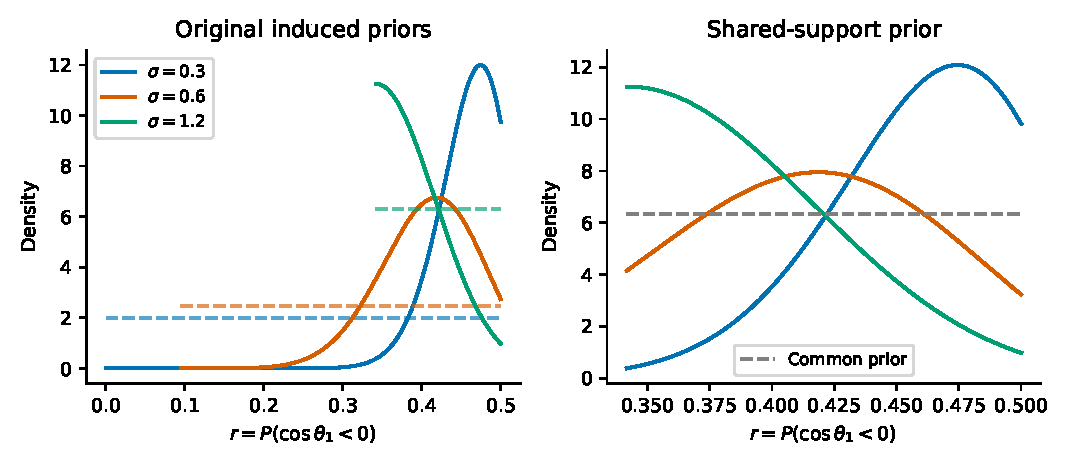
\includegraphics[width=.96\linewidth]{prior-support.pdf}
\caption{Baseline mass, spin-amplitude, and redshift settings are fixed while tilt width varies. Left: r priors and posteriors induced by the original uniform-f prior. Right: the uniform-r control on shared support. Dashed lines show priors. The shared-support control changes the scientific prior; distances between curves do not directly establish physical robustness.}\label{fig:1}
\end{figure}
The common-prior experiment retains 39.06\% of the baseline original prior mass and 84.97\% of its original posterior mass. Its r median becomes 41.87\%, with interval 35.28\%–48.67\%. Across all 81 settings, the smallest retained original posterior mass is only 12.70\%; this substantial truncation must accompany interpretation of the results.

Of the 27 triplets, nine show median-span reductions of 6.24–11.37 percentage points. All nine use Beta(1.5,8.5) spin amplitudes and have no domain where all three models pass the MC thresholds. For the nine Beta(2,5) triplets, spans remain similar, increasing slightly by 0.006–0.090 percentage points. Changes for the nine uniform-amplitude triplets are smaller than 0.00002 percentage points. In total, 12 triplets have no common passing point. Here an empty domain refers to the numerical screen on the specified grid and thresholds.

\begin{figure}[tbp]
\centering
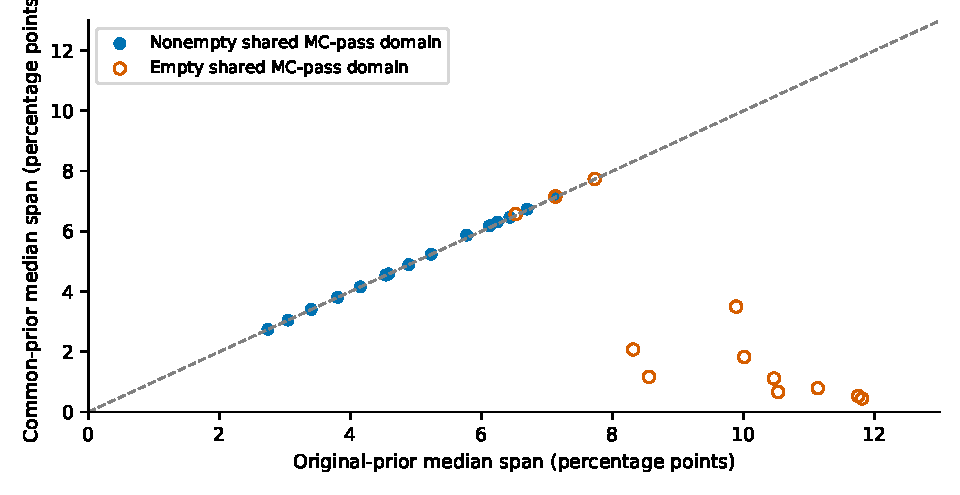
\includegraphics[width=.96\linewidth]{common-prior-groups.pdf}
\caption{Median spans of 27 width triplets before and after matching the r prior. The dashed line marks unchanged span. Open points denote triplets with no common MC-passing domain. All substantially reduced spans are open points. The plot does not remove points or renormalize posteriors using the MC screen.}\label{fig:2}
\end{figure}
\subsection{Paired differences and empirical perturbations}\label{sec:7.2}
In Table~\ref{tab:3}, each difference is the r posterior median of the narrower-\(\sigma\) model minus that of the wider model, in percentage points. The empirical range gives the 5th–95th percentiles when both events and injections are perturbed.

\begin{table}[tbp]
\centering\small
\caption{Paired differences of posterior medians and empirical numerical perturbations (percentage points).}\label{tab:3}
\begin{tabularx}{\linewidth}{Y c c c Y}
\toprule
Spin-amplitude assumption & \(\sigma\) comparison & Original difference & Paired SD & Empirical range \\
\midrule
Beta(1.5,8.5) & 0.3\(-\)0.6 & 0.914 & 0.983 & \(-\)0.188 to 2.958 \\
Beta(1.5,8.5) & 0.3\(-\)1.2 & 1.115 & 1.212 & \(-\)0.293 to 3.601 \\
Beta(1.5,8.5) & 0.6\(-\)1.2 & 0.201 & 0.299 & \(-\)0.198 to 0.758 \\
Beta(2,5) & 0.3\(-\)0.6 & 3.778 & 0.450 & 2.950 to 4.453 \\
Beta(2,5) & 0.3\(-\)1.2 & 6.734 & 0.616 & 5.557 to 7.600 \\
Beta(2,5) & 0.6\(-\)1.2 & 2.956 & 0.370 & 2.309 to 3.521 \\
\bottomrule
\end{tabularx}
\end{table}
\begin{figure}[tbp]
\centering
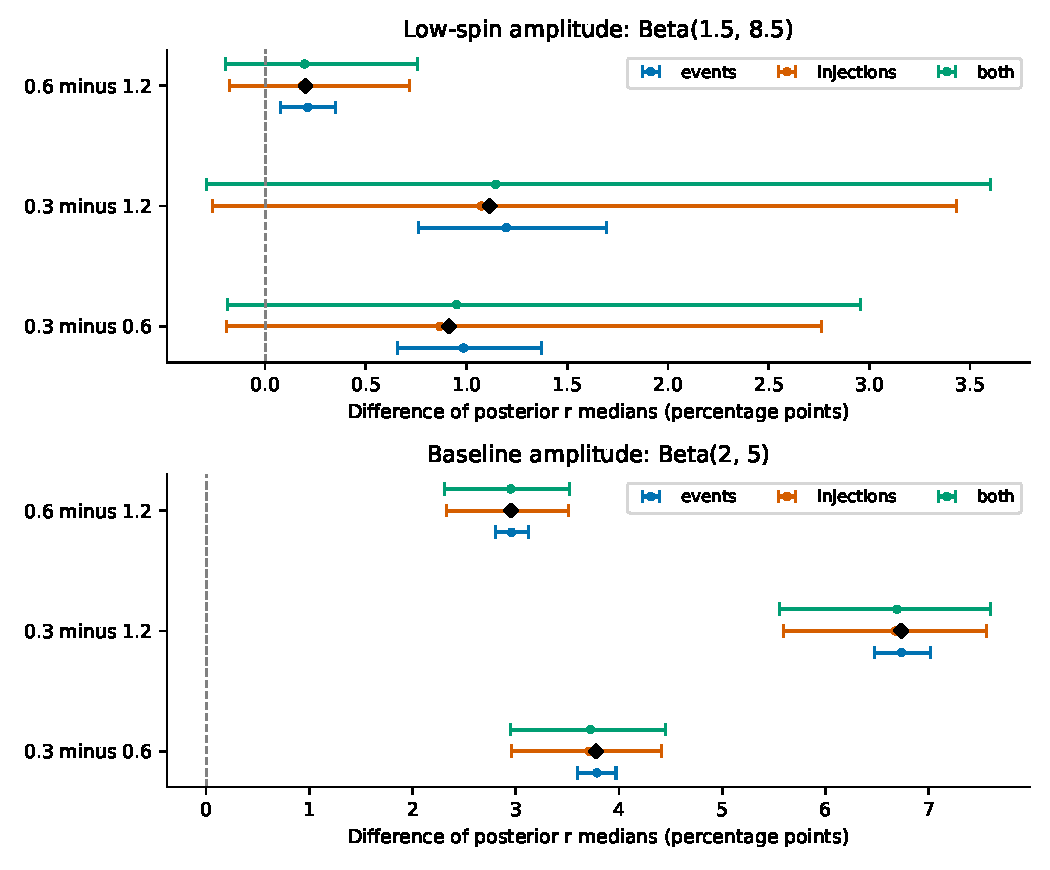
\includegraphics[width=.86\linewidth]{paired-bootstrap.pdf}
\caption{Differences between model medians using shared samples. Points and error bars show empirical resampling medians and 5th–95th percentile ranges; black diamonds indicate original differences. Events, injections, and both are perturbed separately. These intervals describe numerical sensitivity, not probabilities that a model is correct or astrophysical credible intervals.}\label{fig:3}
\end{figure}
Width-model differences under the baseline amplitude assumption persist under this empirical perturbation. Low-spin ranges cross zero, indicating unstable ordering under the specified mechanism; this does not establish model equivalence. Retaining covariance also materially changes the error scale. For the baseline \(\sigma\)=0.3 versus 0.6 comparison, the median-perturbation correlation is approximately 0.812. The paired SD is 0.450 percentage points, compared with 1.035 points if covariance is ignored.

\subsection{Separating event and injection perturbations}\label{sec:7.3}
Table~\ref{tab:4} reports the perturbation SD of each model's r median in percentage points. The three modes share the generated event and injection counts. A full posterior median is nonlinear, so its variance need not be strictly additive.

\begin{table}[tbp]
\centering\small
\caption{Perturbation standard deviations of individual model medians (percentage points).}\label{tab:4}
\begin{tabularx}{\linewidth}{Y c c c Y}
\toprule
Spin-amplitude assumption & \(\sigma\) & Events only & Injections only & Both \\
\midrule
Beta(1.5,8.5) & 0.3 & 0.323 & 1.324 & 1.413 \\
Beta(1.5,8.5) & 0.6 & 0.153 & 0.582 & 0.616 \\
Beta(1.5,8.5) & 1.2 & 0.133 & 0.442 & 0.469 \\
Beta(2,5) & 0.3 & 0.188 & 0.730 & 0.753 \\
Beta(2,5) & 0.6 & 0.165 & 0.689 & 0.710 \\
Beta(2,5) & 1.2 & 0.107 & 0.434 & 0.452 \\
\bottomrule
\end{tabularx}
\end{table}
For these six settings and this empirical mechanism, injection perturbations have the larger effect on the r median. This does not resolve low-ESS events: unobserved tails and event-posterior correlations are outside the mechanism.

In the low-spin \(\sigma\)=0.3 setting, the delta-method posterior-averaged pointwise log-likelihood variance is 3.730, whereas D is approximately 0.254 and its nonlinear empirical value is approximately 0.257. The event contribution has pointwise variance about 0.391 and shape diagnostic about 0.014. These all-event summaries indicate that part of the pointwise error is a relatively large common normalization perturbation with a smaller effect on conditional posterior shape. This decomposition cannot uniquely attribute the cancellation to a particular low-ESS event. Pointwise screens and shape diagnostics must therefore be reported together, rather than substituted for one another.

\FloatBarrier
\section{Independent validation and error classification}\label{sec:8}
Validation covers analytic mathematics, discrete implementation, the empirical stochastic mechanism, and provenance matching. Analytic checks address truncated-Gaussian integrals, functional semantics, and affine information invariance. Discrete checks address likelihood reconstruction, prior recovery under constant likelihood, quadrature, and quantile conventions. Stochastic checks use small synthetic data to test exact covariance and shared counts. Provenance checks verify source-file checksums and elementwise matches.

\begin{table}[tbp]
\centering\small
\caption{Independent numerical validation. Errors are in proportion units unless specified otherwise.}\label{tab:5}
\begin{tabularx}{\linewidth}{YY}
\toprule
Validation item & Maximum error or result \\
\midrule
Affine information invariance across 81 settings & 2.1\(\times\)10\textsuperscript{-15} \\
Conditional quantiles: 4001 versus 8001 points & 3.40\(\times\)10\textsuperscript{-7} \\
Common posterior versus independent conditional integration & 5.30\(\times\)10\textsuperscript{-9} \\
Common-prior recovery under constant likelihood & 2.21\(\times\)10\textsuperscript{-14} \\
Raw-moment recomputation for six settings & Exact agreement \\
Grid refinement for 64 fixed bootstrap samples & 1.78\(\times\)10\textsuperscript{-7} \\
Explicit zero vector versus collapsed covariance & 4.9\(\times\)10\textsuperscript{-17} \\
Full-grid covariance versus Equation~\eqref{eq:14} & 3.6\(\times\)10\textsuperscript{-17} \\
Shared-count cancellation for proportional models & 3.1\(\times\)10\textsuperscript{-15} \\
Independent synthetic resampling & 20000 repetitions; passed \\
\bottomrule
\end{tabularx}
\end{table}
The earlier result uses a 501-point cumulative midpoint CDF; this stage uses endpoint-inclusive trapezoidal quadrature. Quantiles differ by at most 0.1003 percentage points between these conventions, while likelihood densities agree to 2.45\(\times\)10\textsuperscript{-14}. We retain the earlier output and do not interpret the quantile-convention difference as a new physical effect.

A duplicated-sample counterexample copies every row seven times. Treating these copies as independent spuriously reduces the estimated variance to 1/7. Correctly preserving perfect correlation between copies leaves the mean and variance unchanged. Increasing bootstrap repetitions improves estimation of diagnostic quantities, not the independent information in the original events or injections.

These checks do not validate missed tails in the real data, event-prior correctness, the actual campaign sampling design, or the population model. We have not completed simulation calibration or coverage studies based on the true generative workflow.

\FloatBarrier
\section{Discussion}\label{sec:9}
\subsection{Conclusions supported by this study}\label{sec:9.1}
A population functional with consistent semantics across models facilitates comparison, but its induced prior must also be disclosed. A one-to-one transformation at fixed \(\sigma\) adds no information; a shared-support control actively changes the prior. These are different operations. Provenance auditing can exclude specific implementation explanations instead of attributing every discrepancy generically to systematics. Here, restoring near-unity mixture weights cannot explain the model differences. Finally, preserving shared-sample covariance distinguishes width-model differences that persist under empirical perturbations from low-spin cases with unstable ordering.

Each conclusion is conditional. Persistence of the baseline difference shows that model choice still changes r inference under the current common prior, model family, and empirical mechanism. It does not identify the model closest to the real Universe. Low-spin ranges crossing zero show that a fine ordering lacks support from this numerical diagnostic, without establishing identical model predictions.

\subsection{Conclusions that cannot be extrapolated}\label{sec:9.2}
We use one restricted tilt-mixture family, without a joint posterior over free width and other hyperparameters, a general nonparametric tilt distribution, or free mass–tilt and amplitude–tilt correlations. The restriction r\(\leq\)0.5 is imposed by the model, not independently discovered from the data. Formation-channel interpretation additionally requires testable population-synthesis predictions and control of omitted channels and model misspecification \cite{ref1}.

Although the source injection file, finite-sample selection mask, and density transformation are recovered, the full per-event waveform, prior, and identity provenance remains unresolved. Consistency between the tutorial event selection and injection detection protocol is also not sufficiently established. We therefore cannot promote the point estimates or intervals to formal astrophysical measurements, or substitute successful numerical tests for provenance and model validation.

\subsection{Relation to the literature and next steps}\label{sec:9.3}
Earlier studies discuss tilt-distribution model dependence \cite{ref2}, and direct results already exist for angular functionals and larger simulated catalogs \cite{ref5}. Effective-spin degeneracy analyses further caution that inferred component-tilt structure can arise from model extrapolation \cite{ref6}. We do not reproduce effective-spin information-ablation experiments or present a fixed-width scan as such an experiment. Treatment of shared-sample correlated errors follows existing theory \cite{ref3,ref4}. Our contribution is a reproducible diagnostic and provenance repair for explicitly identified inputs.

The next priority is to freeze original PE and search records for each event, then construct an appropriate error model using recovered run labels and the actual generation design. Synthetic-catalog recovery and coverage tests should follow. Only then should the analysis expand to multiple tilt-model families, free hyperparameters, or formation-channel mappings. Upgrading the observing catalog requires freezing the complete combination of posteriors, selection, and versions, rather than merely increasing event count.

\FloatBarrier
\section{Conclusions}\label{sec:10}
On a public 69-event tutorial baseline, we complete prior-support diagnostics for 81 settings, row-level provenance recovery for 41,972 injections, and 2,048 paired empirical resamples for six settings. The 6.734 percentage-point difference between baseline width models persists under this perturbation, whereas the 1.115-point low-spin difference readily changes ordering. The largest computed common-prior median effect of the recovered run-mixture-weight omission is only 6.65\(\times\)10\textsuperscript{-9} and cannot explain these differences.

Matching the target functional, matching prior support, verifying data provenance, and preserving numerical-error covariance are four distinct tasks. Treating them separately avoids mistaking coordinate compression, support truncation, or shared normalization perturbations for new physical information. The result is a publicly inspectable conditional study. Formation-channel fractions still require complete provenance, consistent selection, simulation calibration, and a mapping to physical models.

\FloatBarrier
\section*{Data and code availability}
Original code, manuscripts, figures, and derived statistical results are public with the project. Raw tutorial samples, the large HDF, runtime environments, and upstream documentary snapshots are not redistributed in the repository; public sources, hashes, and reconstruction instructions are retained. All reported numbers are traceable to stage-result JSON files. Random seeds, input hashes, implementation scripts, and independent validation scripts are available. Detailed commands are in \path{research/REPRODUCING_POPULATION.md}.

Publication of the paper and code does not imply completed peer review or endorsement by LVK or the cited authors. AI assistance was used in manuscript preparation and implementation. Numerical results are supported by executable deterministic checks, synthetic tests, source-file matching, and independent implementation cross-checks, not by language-model judgment. No unperformed experiment is reported.

\FloatBarrier
\appendix
\section{Reproduction checklist}\label{app:reproduction}
SHA-256 of the frozen primary input \path{results/model.json}:\par\nopagebreak
\path{6dcf3c9f4fd51b2007977d131c61f69c7d861afb986551ea82b70a7667a51083}

SHA-256 of the official source injection HDF:\par\nopagebreak
\path{81883c571a9fe0b30747c7bc9daca6d358fcd68ef375c7ace0b93aa9ea2e74fe}

\begin{table}[tbp]
\centering\small
\caption{Reproduction entry points for the scientific calculations.}\label{tab:6}
\begin{tabularx}{\linewidth}{YY}
\toprule
Task & Script or result entry point \\
\midrule
Stage-one functionals and prior controls & \path{research/population_functionals.py} \\
Independent stage-one mathematics and quadrature checks & \path{research/test_population_functional_math.py}; \path{research/validate_population_functionals.py} \\
Stage-two paired resampling & \path{research/population_mc_bootstrap.py} \\
Synthetic mechanism and implementation cross-checks & \path{research/validate_population_mc_synthetic.py}; \path{research/validate_population_mc_implementation.py} \\
Row-level injection matching & \path{research/population-stage2/provenance_match_injections.py} \\
Recovered mixture-weight controls & \path{research/population_mixture_weight_control.py} \\
\bottomrule
\end{tabularx}
\end{table}
The main local analysis used Python 3.14, NumPy 2.4.6, SciPy 1.18.0, and Astropy 8.0.1. A separate adapter environment was used for mathematical and provenance cross-checks. Figure/PDF dependencies are listed separately from scientific-computation dependencies. Error tolerances, the stochastic mechanism, and the pre-implementation design of the shared-support control are retained in the repository.

\FloatBarrier
\begingroup\small
\setlength{\bibsep}{2pt}
\begin{thebibliography}{99}
\bibitem{ref1} Zevin M., et al. One Channel to Rule Them All? Constraining the Origins of Binary Black Holes Using Multiple Formation Pathways. 2020. \href{https://arxiv.org/abs/2011.10057}{arXiv:2011.10057}.
\bibitem{ref2} Vitale S., Biscoveanu S., Talbot C. Spin it as you like: The (lack of a) measurement of the spin tilt distribution with LIGO-Virgo-KAGRA binary black holes. 2022. \href{https://arxiv.org/abs/2209.06978v3}{arXiv:2209.06978v3}.
\bibitem{ref3} Essick R., Farr W. Precision Requirements for Monte Carlo Sums within Hierarchical Bayesian Inference. 2022. \href{https://arxiv.org/abs/2204.00461v1}{arXiv:2204.00461v1}.
\bibitem{ref4} Talbot C., Golomb J. Growing Pains: Understanding the Impact of Likelihood Uncertainty on Hierarchical Bayesian Inference for Gravitational-Wave Astronomy. 2023. \href{https://arxiv.org/html/2304.06138v2}{arXiv:2304.06138v2}.
\bibitem{ref5} Vitale S., Mould M. The Long Road to Alignment: Measuring Black Hole Spin Orientation with Expanding Gravitational-Wave Datasets. 2025. \href{https://arxiv.org/html/2505.14875v2}{arXiv:2505.14875v2}.
\bibitem{ref6} Wolfe N. E., Hussain A., Heinzel J., Vitale S. Binary-black hole spin population results may be driven by prior degeneracies. 2026. \href{https://arxiv.org/html/2609.10753v1}{arXiv:2609.10753v1}.
\bibitem{ref7} Talbot C., et al. Population inference on GWTC-3, GWPopulation example notebook. \href{https://colmtalbot.github.io/gwpopulation/examples/GWTC3.html}{Official tutorial}; \href{https://github.com/ColmTalbot/gwpopulation/blob/2daa71e8c56362f2f64e2166a0055478557f239a/examples/GWTC3.ipynb}{commit-pinned source}. Source history and access records are retained with this study.
\bibitem{ref8} LIGO Scientific Collaboration, Virgo Collaboration, KAGRA Collaboration. O1+O2+O3 Search Sensitivity Estimates. \href{https://zenodo.org/records/7890398}{Zenodo record 7890398}; \href{https://zenodo.org/records/5636816}{historical record 5636816} for the corresponding HDF. Specific authorship and licensing follow the data-release records.
\bibitem{ref9} Essick R. Constructing Mixture Models for Sensitivity Estimates from Subsets of Separate Injections. Research Notes of the AAS, 5(10), 220, 2021. \href{https://doi.org/10.3847/2515-5172/ac2ba7}{DOI:10.3847/2515-5172/ac2ba7}.
\end{thebibliography}
\endgroup
\end{document}
